\section{Aplicaciones}

\subsection{}

\begin{frame}[c]\frametitle{Introducción}		
	
	\begin{columns}[c]
		\hspace{-5mm}
		\begin{column}{0.45\textwidth}
			\begin{figure}
				\centering
				\begin{subfigure}[b]{0.4\textwidth}
					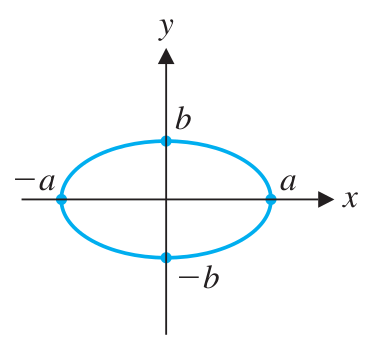
\includegraphics[width=1.4\textwidth]{imagenes/elipse1}
					\caption{$a>b$}
				\end{subfigure}
				\qquad 
				~ %add desired spacing between images, e. g. ~, \quad, \qquad, \hfill etc. 
				%(or a blank line to force the subfigure onto a new line)
				\begin{subfigure}[b]{0.4\textwidth}
					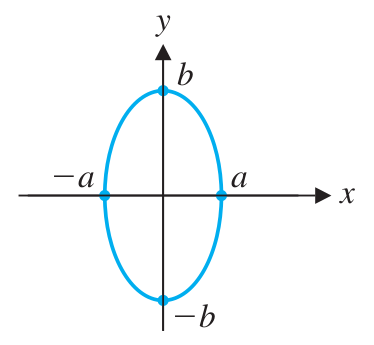
\includegraphics[width=1.4\textwidth]{imagenes/elipse2}
					\caption{$a<b$}
				\end{subfigure}
				\vspace{3mm}
				\caption{$\dfrac{x^2}{a^2}+\dfrac{y^2}{b^2}=1$}
			\end{figure}
		\end{column}
		\hspace{6mm}
		\begin{column}{0.45\textwidth}
			\begin{figure}
				\centering
				\begin{subfigure}[b]{0.4\textwidth}
					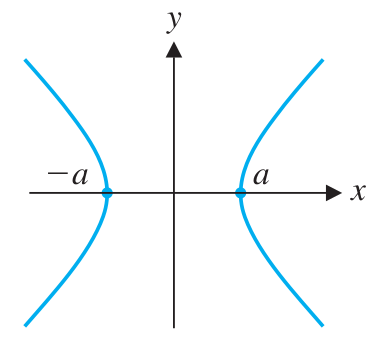
\includegraphics[width=1.4\textwidth]{imagenes/hiperbola1}					
					\caption{$a, b>0$}
				\end{subfigure}
				\qquad 
				~ %add desired spacing between images, e. g. ~, \quad, \qquad, \hfill etc. 
				%(or a blank line to force the subfigure onto a new line)
				\begin{subfigure}[b]{0.4\textwidth}
					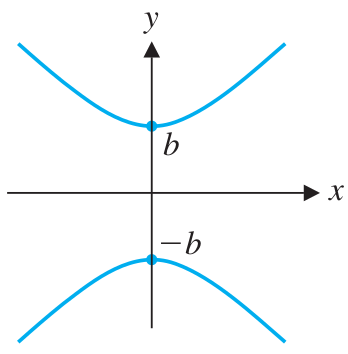
\includegraphics[width=1.4\textwidth]{imagenes/hiperbola2}
					\caption{$a, b>0$}
				\end{subfigure}
				\vspace{3mm}
				\caption{$\dfrac{x^2}{a^2}-\dfrac{y^2}{b^2}=1$}
			\end{figure}	
		\end{column}
	\end{columns}	
\end{frame}

%%------------------------------------------------------------------------------------------------------


\subsection{}

{\nologo 
\begin{frame}\frametitle{Formas cuadráticas}

\begin{columns}[c]
    	\hspace{8mm}
		\begin{column}{0.45\textwidth}
			\begin{figure}
				\centering
				\begin{subfigure}[b]{\textwidth}
					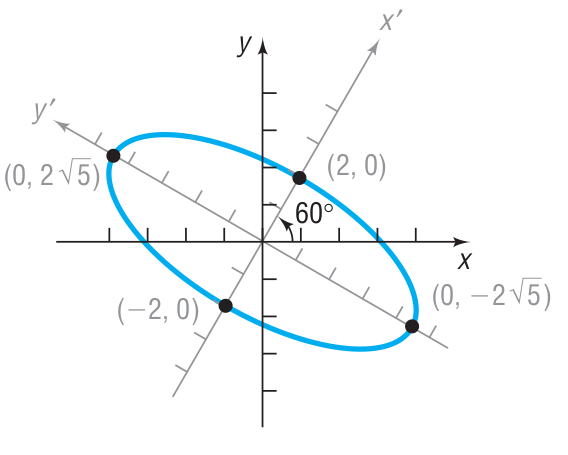
\includegraphics[width=0.93\textwidth]{imagenes/elipse3}
					%\caption{$a>b$}
				\end{subfigure}			
				\vspace{0mm}
				\caption{$x^2+\sqrt{3}\,xy+2y^2=10$}
			\end{figure}
		\end{column}
		\hspace{8mm}
		\begin{column}{0.45\textwidth}
			\begin{figure}
				\centering
				\begin{subfigure}[b]{\textwidth}
					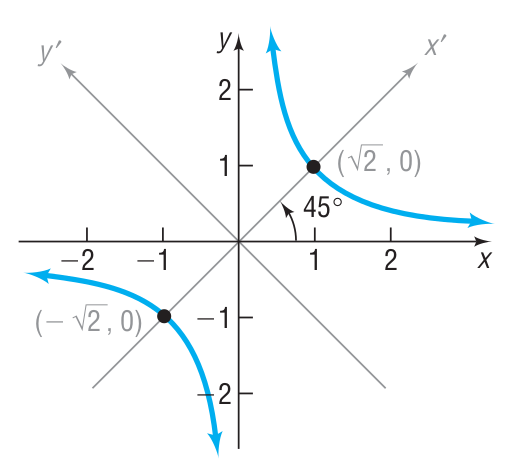
\includegraphics[width=0.8\textwidth]{imagenes/hiperbola3}					
					%\caption{$a, b>0$}
				\end{subfigure}				
				\vspace{0mm}
				\caption{$xy=1$}
			\end{figure}	
		\end{column}
\end{columns}	

\vspace{-1mm}
\begin{block}{\textbf{Definición 1 (Forma cuadrática)}}
	\justifying
	Una expresión de la forma
	\[
	ax^2+cxy+by^2
	\]
	se llama \textbf{\textit{forma cuadrática}} en las variables $x$ y $y$. 
\end{block}

\end{frame}
}

%%------------------------------------------------------------------------------------------------------

\subsection{}

\begin{frame}\frametitle{Ejemplos}

\begin{enumerate}
	\item $4x^2 +9y^2 = \left(\begin{array}{cc} x &y \end{array}\right) \left(\begin{array}{cc}4&0\\[1mm]0&9\end{array}\right) \left(\begin{array}{c}x\\[1mm] y\end{array}\right)$% = 36$
	
	\vspace{5mm}
	\item $5x^2 +2y^2 = \left(\begin{array}{cc} x &y \end{array}\right) \left(\begin{array}{cc}5&0\\[1mm]0&2\end{array}\right) \left(\begin{array}{c}x\\[1mm] y\end{array}\right)$% = 10$
	
	\vspace{5mm}
	\item $2x^2 - 3y^2 = \left(\begin{array}{cc} x &y \end{array}\right) \left(\begin{array}{cc}2&0\\[1mm]0&-3\end{array}\right) \left(\begin{array}{c}x\\[1mm] y\end{array}\right)$% = 1$
	
	\vspace{5mm}
	\item $5x^2 +4xy+3y^2 = \left(\begin{array}{cc} x &y \end{array}\right) \left(\begin{array}{cc}5&2\\[1mm]2&3\end{array}\right) \left(\begin{array}{c}x\\[1mm] y\end{array}\right)$% = 6$
	
	\vspace{5mm}
	\item $5x^2 + 14xy-3y^2 = \left(\begin{array}{cc} x &y \end{array}\right) \left(\begin{array}{rr}5&7\\[1mm]7&-3\end{array}\right) \left(\begin{array}{c}x\\[1mm] y\end{array}\right)$% = 6$
\end{enumerate}

\end{frame}


%%------------------------------------------------------------------------------------------------------

\subsection{}

{\nologo
\begin{frame}%\frametitle{Representación matricial de formas cuadráticas}

\begin{prop}{\textbf{Propiedad 1 (Representación matricial de formas cuadráticas)}}
	\[
	ax^2 + cxy + by^2 =
	\left(
	\begin{array}{@{\hspace{0.3\tabcolsep}}c@{\hspace{\tabcolsep}}c@{\hspace{0.3\tabcolsep}}}
	x & y  
	\end{array}
	\right)
	\left(
	\begin{array}{cc}
	a & c/2   \\[2mm]
	c/2 & b
	\end{array}
	\right)
	\left(
	\begin{array}{@{\hspace{0.5\tabcolsep}}c@{\hspace{0.5\tabcolsep}}}
	x   \\[1mm]
	y
	\end{array}
	\right)
	=
	\mathbf{x}^T A\, \mathbf{x}
	\]
\end{prop}

\vspace{2mm}
\begin{enumerate}
	\item[\labelname{6}] $4x^2 +9y^2 = \left(\begin{array}{cc} x &y \end{array}\right) \left(\begin{array}{cc}4&0\\[1mm]0&9\end{array}\right) \left(\begin{array}{c}x\\[1mm] y\end{array}\right)$% = 10$
			
	\vspace{3mm}
	\item[\labelname{7}] $13x^2 -10xy+13y^2 = \left(\begin{array}{cc} x &y \end{array}\right) \left(\begin{array}{rr}13&-5\\[1mm]-5&13\end{array}\right) \left(\begin{array}{c}x\\[1mm] y\end{array}\right)$% = 6$	
\end{enumerate}

\vspace{-1mm}
\begin{alertblock}{\textbf{Observación 1}}
	\begin{enumerate}[$a$]\justifying 
		\item Formas cuadráticas asociadas a matrices diagonales no tienen ``términos cruzados'' $xy$.
		\item La matriz $A$ asociada a una forma cuadrática es simétrica.
		\item Toda matriz simétrica real se puede diagonalizar ortogonalmente.
		\item En toda forma cuadrática es posible eliminar los ``términos cruzados'' $xy$, 
		mediante un cambio de variables adecuado.
	\end{enumerate}
\end{alertblock}	

\end{frame}
}

%%------------------------------------------------------------------------------------------------------

\subsection{} 

{\nologo 
\begin{frame}\frametitle{Diagonalización de una forma cuadrática}
	
	\[
	A \text{ simétrica } \quad  \Longrightarrow \quad A = QDQ^T, \ \text{ con } Q \text{ ortogonal.}
	\]
	
	\smallskip
	\[
	%\mathbf{x} = Q\mathbf{y} \quad  \Longrightarrow \quad 	
	\mathbf{x}^TA \mathbf{x} \ = \
	\mathbf{x}^T\left(QDQ^T \right) \mathbf{x} \ = \
	%\left(Q\mathbf{x}\right)^TD\left(Q\mathbf{x}\right) \ = \
	\left(Q^T\mathbf{x}\right)^T D\left(Q^T\mathbf{x}\right) \ = \
	%\mathbf{y}^TQ^TA Q\mathbf{y} = 
	\mathbf{x'}^TD\, \mathbf{x'}
	\]
	
	\vspace{0mm}
	\begin{alertblock}{\textbf{Observación 1}}
		El cambio de variable $\mathbf{x} = Q\mathbf{x'}$ es una rotación de ejes que permite eliminar los términos 
		cruzados $xy$ en la forma cuadrática $\mathbf{x}^TA \mathbf{x}$.
	\end{alertblock}	
	
	\vspace{0mm}
	\begin{prop}{\textbf{Propiedad 2 (Teorema de los ejes principales)}}\justifying 
		Si $A$ es la matriz simétrica $2\times 2$ asociada a una forma cuadrática $\mathbf{x}^TA \mathbf{x}$ 
		y si $Q$ es una matriz ortogonal tal que $Q^TAQ = D$ es una matriz diagonal, entonces el cambio de variable $\mathbf{x}=Q\mathbf{x'}$ transforma la forma cuadrática en
		\[
		\mathbf{x}^TA \mathbf{x} = 
		%\mathbf{x'}^TQ^TAQ\, \mathbf{x'} =
		\left(
		\begin{array}{@{\hspace{0.3\tabcolsep}}c@{\hspace{\tabcolsep}}c@{\hspace{0.3\tabcolsep}}}
		x' & y'  
		\end{array}
		\right)
		\left(
		\begin{array}{@{\hspace{0.3\tabcolsep}}c@{\hspace{1.2\tabcolsep}}c@{\hspace{0.3\tabcolsep}}}
		\lambda_1 & 0   \\[2mm]
		0 & \lambda_2
		\end{array}
		\right)
		\left(
		\begin{array}{@{\hspace{0.5\tabcolsep}}c@{\hspace{0.5\tabcolsep}}}
		x'   \\[1mm]
		y'
		\end{array}
		\right)
		=				
		%\mathbf{y}^TD \mathbf{y} = 
		\lambda_1\left(x'\right)^2 + \lambda_2\left(y'\right)^2
		\]
	\end{prop}
	
\end{frame}
}

%%%------------------------------------------------------------------------------------------------------
%
%\subsection{} 
%
%\begin{frame}\frametitle{Diagonalización de una forma cuadrática}
%
%\[
%A \text{ simétrica } \quad  \Longrightarrow \quad Q^TAQ = D, \ \text{ con } Q \text{ ortogonal.}
%\]
%
%\smallskip
%\[
%\mathbf{x} = Q\mathbf{y} \quad  \Longrightarrow \quad 	
%\mathbf{x}^TA \mathbf{x} = \left(Q\mathbf{y}\right)^TA \left(Q\mathbf{y}\right) 
%= \mathbf{y}^TQ^TA Q\mathbf{y} = \mathbf{y}^TD \mathbf{y}
%\]
%
%\medskip
%\begin{alertblock}{\textbf{Observación 2}}
%	El cambio de variable $\mathbf{x} = Q\mathbf{y}$ es una rotación de ejes que permite eliminar los términos 
%	cruzados $xy$ en la forma cuadrática $\mathbf{x}^TA \mathbf{x}$.
%\end{alertblock}	
%
%%\vspace{5mm}
%\medskip
%\begin{prop}{\textbf{Teorema (de los ejes principales)}}\justifying 
%Toda forma cuadrática puede diagonalizarse. Específicamente, si $A$ es la matriz simétrica $n\times n$, 
%asociada a la forma cuadrática $\mathbf{x}^TA \mathbf{x}$, y si $Q$ es una matriz ortogonal
%tal que $Q^TAQ = D$ es una matriz diagonal, entonces el cambio de variable $\mathbf{x}=Q\mathbf{y}$
%transforma la forma cuadrática $\mathbf{x}^TA \mathbf{x}$ en la forma cuadrática $\mathbf{y}^TD \mathbf{y}$,
%que no tiene términos en $xy$. Si los eigenvalores de A son $\lambda_1,\hdots,\lambda_n$ y 
%$\mathbf{y} = [y_1,\hdots,y_n]^T$, entonces
%\[
%	\mathbf{x}^TA \mathbf{x} = \mathbf{y}^TD \mathbf{y} = \lambda_1y_1^2 + \cdots + \lambda_ny_n^2
%\]
%\end{prop}
%
%\end{frame}

%%------------------------------------------------------------------------------------------------------

\subsection{}

\begin{frame}\frametitle{Diagonalización de cónicas}

\begin{ej}{\textbf{Ejemplo 1}} \justifying
	Encuentre un cambio de variable que transforme la forma cuadrática
	\[
		5x^2 + 4xy + 2y^2
	\]
	en una sin términos cruzados en $xy$.
\end{ej}

\end{frame}

%%------------------------------------------------------------------------------------------------------

\subsection{} 

\begin{frame}\frametitle{Matrices ortogonales $2\times 2$}
	
	% https://en.wikipedia.org/wiki/Orthogonal_matrix#Lower_dimensions
	% https://books.google.com.co/books?id=J4FwdwtfmPAC&lpg=PA388&ots=MU7RYnccXG&dq=Demuestre%20que%20una%20matriz%20ortogonal%20de%202%20%20%202%20debe%20tener%20la%20forma&hl=es&pg=PA388#v=onepage&q&f=false
	\begin{prop}{\textbf{Propiedad 3}}\justifying 
		Si $A$ es una matriz ortogonal de $2\times 2$, entonces 
		\begin{figure}
			\centering
			\begin{subfigure}[b]{0.4\textwidth}
				\[
				A=
				\left(
				\begin{array}{@{\hspace{0.5\tabcolsep}}r@{\hspace{1.5\tabcolsep}}r@{\hspace{0.7\tabcolsep}}}
				\cos\theta & -\sen\theta   \\[2mm]
				\sen\theta & \cos\theta  
				\end{array}
				\right)		
				\]
				\caption{Rotación}
			\end{subfigure}
			\hspace{3mm}
			\begin{subfigure}[b]{0.1\textwidth}
				ó
				\vspace{1.15cm}
			\end{subfigure}
			\hspace{-6mm}
			~ %add desired spacing between images, e. g. ~, \quad, \qquad, \hfill etc. 
			%(or a blank line to force the subfigure onto a new line)
			\begin{subfigure}[b]{0.4\textwidth}
				\[
				A=
				\left(
				\begin{array}{@{\hspace{0.5\tabcolsep}}r@{\hspace{1.5\tabcolsep}}r@{\hspace{0.7\tabcolsep}}}
				\cos\theta & \sen\theta   \\[2mm]
				\sen\theta & -\cos\theta  
				\end{array}
				\right)		
				\]
				\caption{Reflexión}
			\end{subfigure}
		\end{figure}
	
		\vspace{2mm}
		para algún $0\leq \theta <2\pi$. Además, $A$ corresponde a una rotación en $\r^2$ si $\det A=1$ y $A$ corresponde 
		a una reflexión en $\r^2$ si $\det A=-1$.
		
	\end{prop}
	
\end{frame}


%%------------------------------------------------------------------------------------------------------

\subsection{}

\begin{frame}\frametitle{Diagonalización de cónicas}
	
	\begin{ej}{\textbf{Ejemplo 2}} \justifying
		Identifique y grafique de la cónica cuya ecuación es
		\[
			5x^2 + 4xy + 2y^2 = 6.
		\]
	\end{ej}
	
\end{frame}

%%------------------------------------------------------------------------------------------------------


\subsection{}

\begin{frame}%\frametitle{Gráfica de ecuaciones cuadráticas}
	
	\begin{block}{\textbf{Definición 2 (Ecuación cuadrática general)}}
		\justifying
		La forma general de una \textit{ecuación cuadrática} en dos variables $x$ y $y$ es
		\[
			ax^2+cxy+by^2 + dx + ey + f= 0,
		\]
		donde al menos uno de los coeficientes $a$, $b$ y $c$ es distinto de cero.
	\end{block}
	
	\vspace{1mm}
	\begin{alertblock}{\textbf{Observación 2}}\justifying 
		La gráfica de una ecuación cuadrática en dos variables corresponde a una sección cónica (que puede ser degenerada).
	\end{alertblock}	

	\begin{figure}		
		\begin{subfigure}[b]{0.22\textwidth}
			\centering
			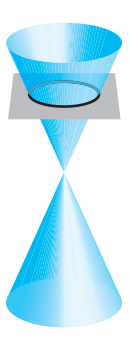
\includegraphics[height=\textwidth]{imagenes/conica1}
			\caption{Circunferencia}
		\end{subfigure}
		\hspace{2mm}
		\begin{subfigure}[b]{0.22\textwidth}
			\centering
			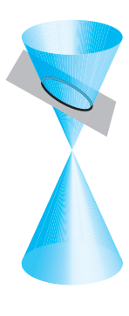
\includegraphics[height=\textwidth]{imagenes/conica2}
			\caption{Elipse}
		\end{subfigure}
		\hspace{2mm}
		\begin{subfigure}[b]{0.22\textwidth}
			\centering
			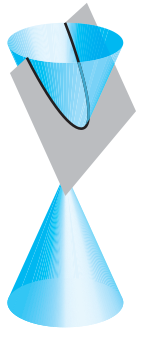
\includegraphics[height=\textwidth]{imagenes/conica3}
			\caption{Parábola}
		\end{subfigure}
		\hspace{2mm}
		\begin{subfigure}[b]{0.22\textwidth}
			\centering
			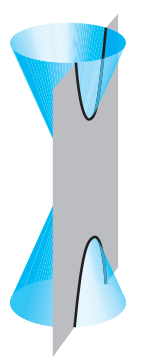
\includegraphics[height=\textwidth]{imagenes/conica4}
			\caption{Hipérbola}
		\end{subfigure}
		\vspace{3mm}
		\caption{Secciones cónicas (no degeneradas)}
	\end{figure}

\end{frame}

%%------------------------------------------------------------------------------------------------------

\subsection{}

{\nologo 
\begin{frame}\frametitle{Secciones cónicas rotadas y trasladadas}
		
		\vspace{-1mm}		
		\begin{prop}{\textbf{Propiedad 4 (Representación matricial de formas cuadráticas)}}
			La expresión cuadrática 
			\[
			ax^2+cxy+by^2 + dx + ey + f
			\]
			se puede escribir en forma matricial como
			\[
			\left(
			\begin{array}{@{\hspace{0.3\tabcolsep}}c@{\hspace{\tabcolsep}}c@{\hspace{0.3\tabcolsep}}}
			x & y  
			\end{array}
			\right)
			\left(
			\begin{array}{cc}
			a & c/2   \\[2mm]
			c/2 & b
			\end{array}
			\right)
			\left(
			\begin{array}{@{\hspace{0.5\tabcolsep}}c@{\hspace{0.5\tabcolsep}}}
			x   \\[1mm]
			y
			\end{array}
			\right)
			+
			\left(
			\begin{array}{@{\hspace{0.3\tabcolsep}}c@{\hspace{\tabcolsep}}c@{\hspace{0.3\tabcolsep}}}
			d & e  
			\end{array}
			\right)
			\left(
			\begin{array}{@{\hspace{0.5\tabcolsep}}c@{\hspace{0.5\tabcolsep}}}
			x   \\[1mm]
			y
			\end{array}
			\right)
			+ f
			=
			\mathbf{x}^T A\, \mathbf{x} +
			B\mathbf{x} + f
			\]
		\end{prop}
				
		\vspace{-1mm}
		\begin{prop}{\textbf{Propiedad 5 (Teorema de los ejes principales - versión 2)}}\justifying 
			Considere la sección cónica
			\[
				\mathbf{x}^T A\, \mathbf{x} + B\mathbf{x} + f = 0.
			\]
			Si $Q$ es una matriz ortogonal tal que $Q^TAQ = D$ es una matriz diagonal, entonces 
			el cambio de variable $\mathbf{x}=Q\mathbf{x'}$ transforma la sección cónica en
			\[
			\mathbf{x}^TA \mathbf{x} +  B\mathbf{x} + f= 
			\lambda_1\left(x'\right)^2 + \lambda_2\left(y'\right)^2 + BQ\mathbf{x'} + f = 0
			\]
		\end{prop}
		
\end{frame}
}

%%------------------------------------------------------------------------------------------------------

\subsection{}

{\nologo 
\begin{frame}\frametitle{Procedimiento para aplicar el teorema de los ejes principales}
	
	\begin{ejem}{\textbf{Procedimiento}}\justifying		
		\begin{enumerate}\justifying
			\item Considere la matriz simétrica $A$ de la sección cónica y halle sus valores propios $\lambda_1$
			y $\lambda_2$.
			\item Halle los vectores propios correspondientes a $\lambda_1$ y $\lambda_2$. Normalice estos vectores
			para formar la matriz $Q$.			
			\item Si $\det Q=-1$, intercambie las columnas de $Q$ para que de esta forma $\det Q=1$ y así
			\[
			Q=
			\left(
			\begin{array}{@{\hspace{0.5\tabcolsep}}r@{\hspace{1.5\tabcolsep}}r@{\hspace{0.7\tabcolsep}}}
			\cos\theta & -\sen\theta   \\[2mm]
			\sen\theta & \cos\theta  
			\end{array}
			\right)		
			\]
			\item El ángulo $\theta$ representa el ángulo de rotación de la cónica.
			\item La ecuación de la cónica rotada es
			\[
				\lambda_1\left(x'\right)^2 + \lambda_2\left(y'\right)^2 + BQ\mathbf{x'} + f = 0
			\]
		\end{enumerate}
	\end{ejem}		
	
\end{frame}
}

%%------------------------------------------------------------------------------------------------------

\subsection{}

\begin{frame}\frametitle{Secciones cónicas rotadas y trasladadas}
	
	\begin{ej}{\textbf{Ejemplo 3}} \justifying
		Identifique y grafique de la cónica cuya ecuación es
		\[
		3x^2 - 10xy + 3y^2 + 16\sqrt{2}\,x - 32 = 0.
		\]
	\end{ej}
	
\end{frame}

%%------------------------------------------------------------------------------------------------------

\subsection{}

\begin{frame}\frametitle{Secciones cónicas rotadas y trasladadas}
	
	\begin{prop}{\textbf{Propiedad 6}}\justifying 
		Considere la sección cónica rotada		
		\[
			\lambda_1\left(x'\right)^2 + \lambda_2\left(y'\right)^2 + BQ\mathbf{x'} + f = 0.
		\]
		
		\vspace{-0mm}
		\begin{enumerate}[$a$]\justifying 
			\item Si $\lambda_1$ y $\lambda_2$ son ambos positivos, o son ambos negativos, la gráfica es una elipse.
			\item Si $\lambda_1=\lambda_2$, la gráfica es una circunferencia.
			\item Si $\lambda_1$ y $\lambda_2$ son de signos opuestos, la gráfica es una hipérbola o 
			dos rectas que se cortan.
			\item Si $\lambda_1=0$ ó $\lambda_2=0$, la gráfica es una parábola, dos rectas que se cortan
			o una sección cónica degenerada.
		\end{enumerate}
	\end{prop}
	
\end{frame}
